\documentclass{beamer}
\usepackage{pgfpages}
\usepackage{newtxtext,newtxmath} %time new roman
%\setbeameroption{show notes}
%\setbeameroption{show notes on second screen=right}
\usetheme{Warsaw}
\usepackage[french]{babel}

\usepackage{tikz}
\pgfdeclareimage[height=0.5cm]{le-logo}{}
%\setbeamertemplate{footline}[frame number]
%Set number slide 

\usepackage[backend=biber]{biblatex}
%\usepackage[backend=biber, style=chem-acs]{biblatex}
\addbibresource{presentation.bib} 
\bibliography{Skin Cancer Detection}
\setbeamertemplate{bibliography item}[triangle]

\usepackage{multirow}% row fusion
\usepackage{array} % column fusion
\usepackage{xfrac} % small fractions
\usepackage{adjustbox}
\usepackage{listings}
\usepackage{color}
\definecolor{gray}{rgb}{0.4,0.4,0.4}
\definecolor{darkblue}{rgb}{0.0,0.0,0.6}
\definecolor{cyan}{rgb}{0.0,0.6,0.6}
 \titlegraphic{\vspace{-1cm}
      \includegraphics[width=2.5cm]{images/paris8_1}\hspace*{4.75cm}~%
      \hfill
      \includegraphics[width=2.5cm]{images/logo}
}
\setbeamertemplate{frametitle}{\nointerlineskip  
    \begin{beamercolorbox}[wd=\paperwidth,ht=2.75ex,dp=1.375ex]{frametitle}
        \hspace*{2ex}\insertframetitle \hfill {\small\insertframenumber/\inserttotalframenumber} \hspace*{1ex}%
    \end{beamercolorbox}}

\usecolortheme{wolverine}
\setbeameroption{hide notes} % Only slides


%%%%%%%%%%%%%%%%%%%%%%%%%%%
\title[Détection du Cancer de la peau] 
{Détection du Cancer de la peau à partir du Convolutional Neural Network}
%\subtitle {ne compléter que si l'article possède un sous-titre}
\author[Komlan Dantodji] 
{Komlan Jean-Marie DANTODJI}

\institute[]
{
  Etudiant en M1 Big Data
  \and
  Université Paris 8}
\date{Dimanche, 24 janvier 2021}


\begin{document}
\begin{frame}
  \titlepage
\end{frame}

\begin{frame}{Plan}
  \tableofcontents
\end{frame}

\section{Introduction}
\begin{frame}{Cancer de la peau}
\begin{figure}[H]
    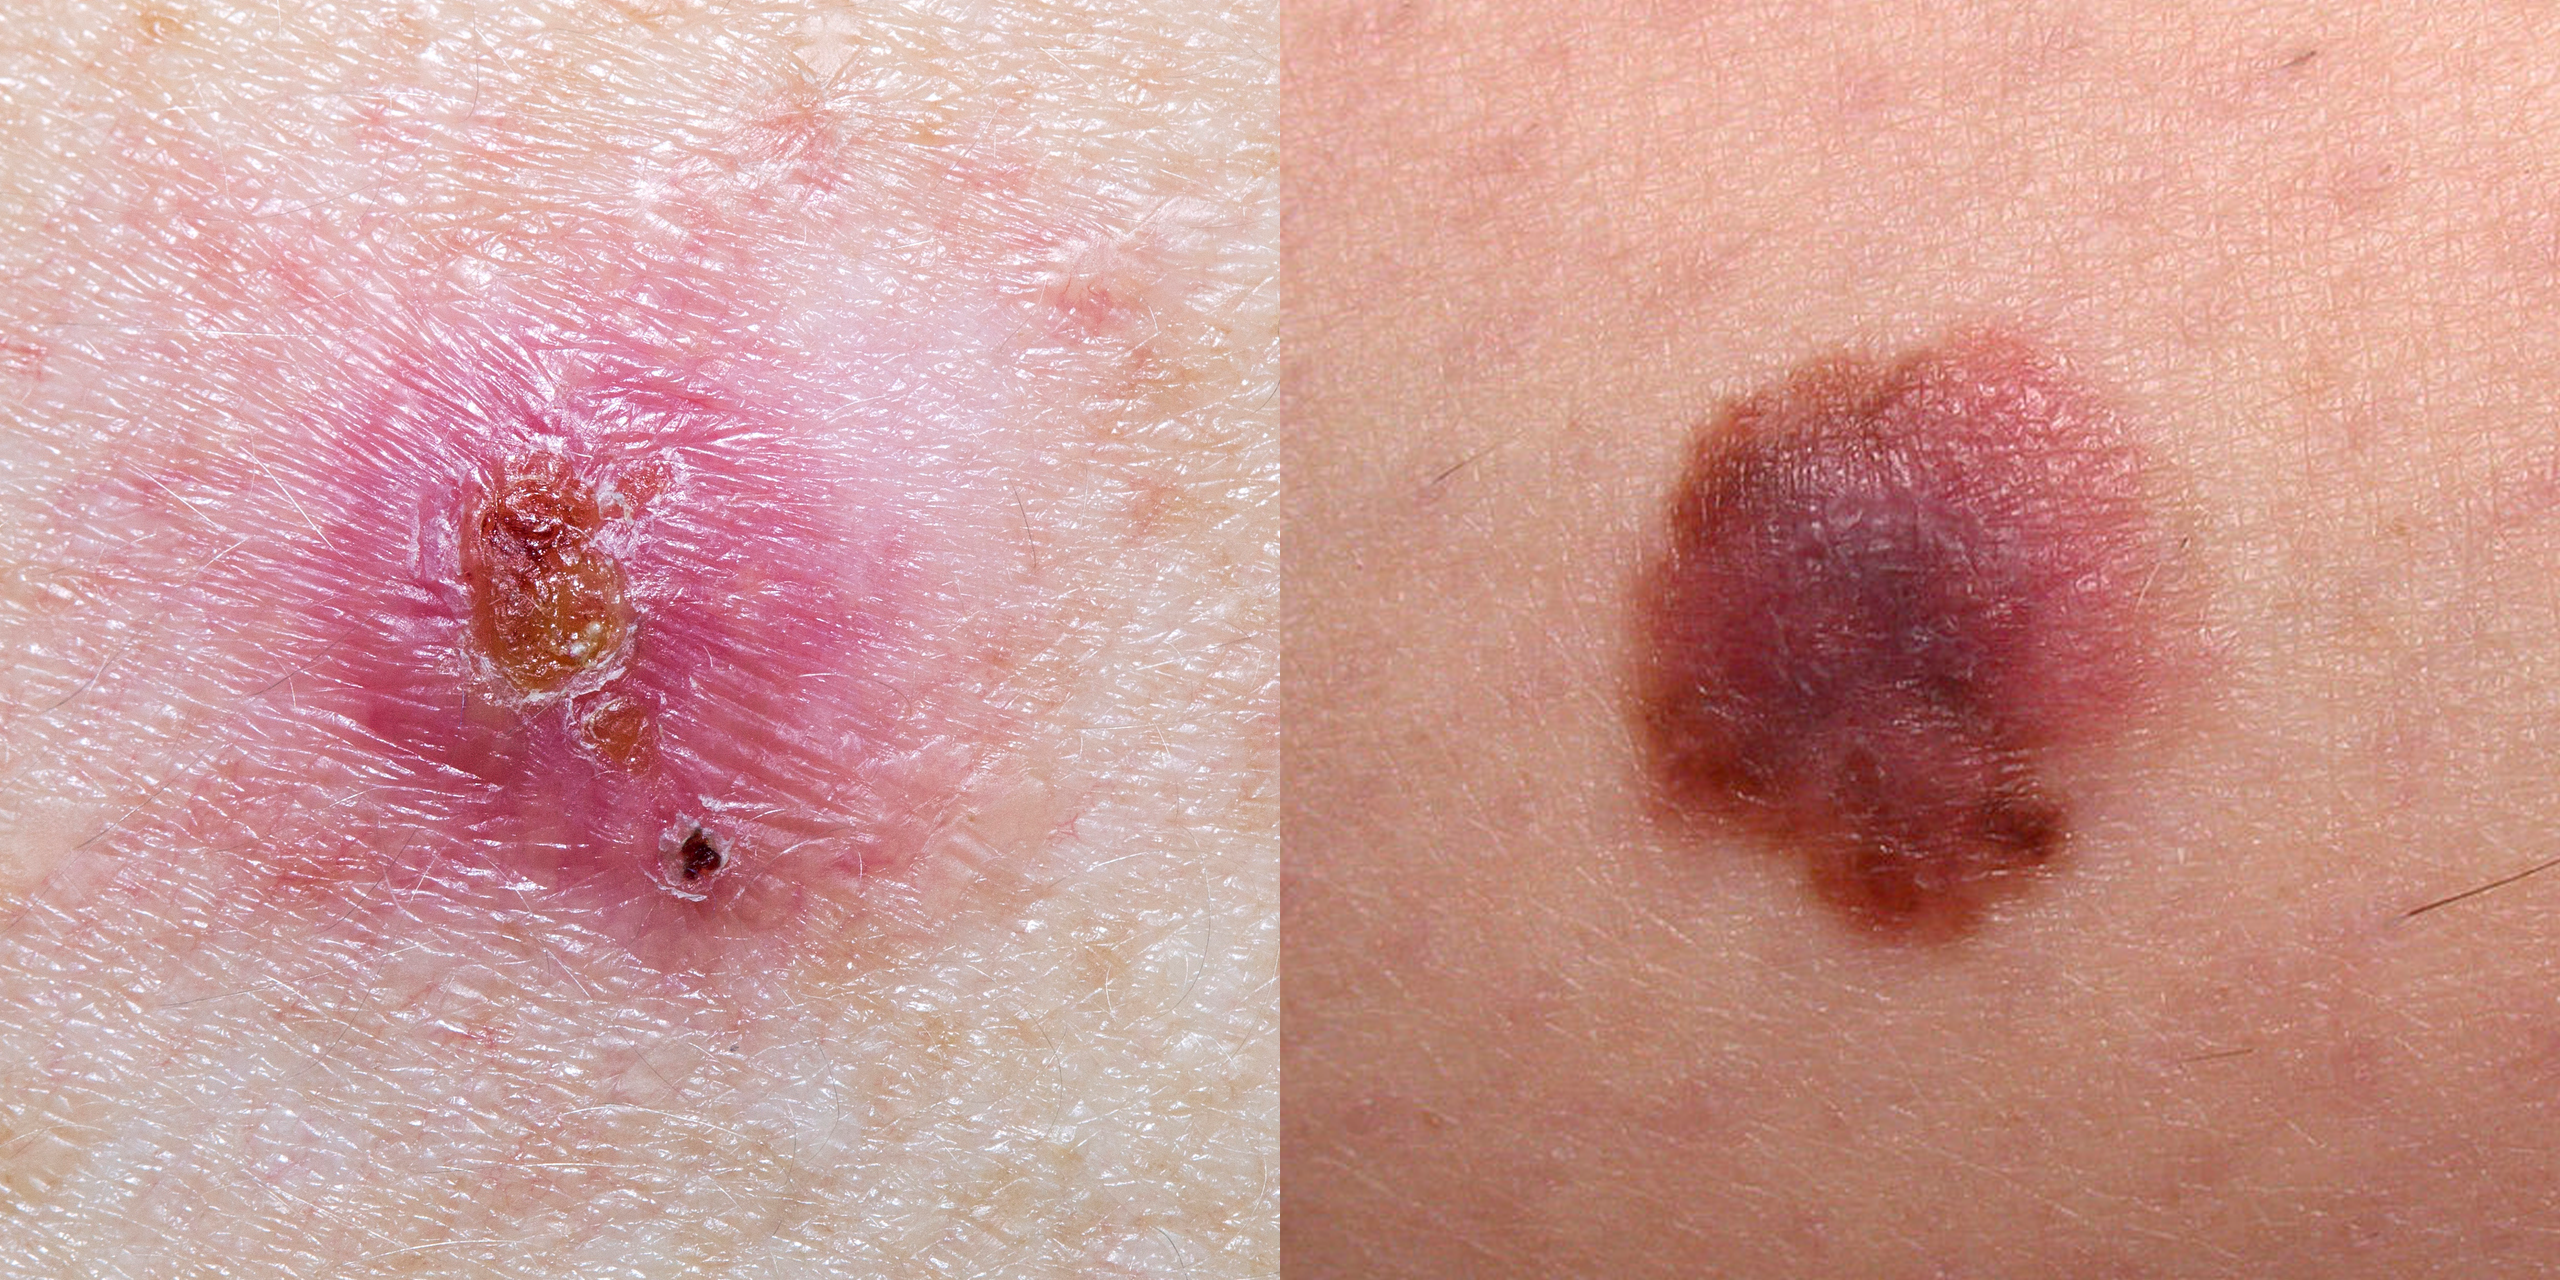
\includegraphics[width=8cm,height=4cm]{images/cancer.png}
    \caption{ Skin Cancer: Google}
    \label{fig:L1}
\end{figure}
\end{frame}

\section{Problématique}
\begin{frame}{Problématique}
\begin{itemize}
		\item Trouver un moyen pour diagnostiquer les cellules cancéreuses dans une image
		\item Faire un prétraitement de l'image
		\item Extraire des caractéristiques dans une image
		\item Appliquer le model du CNN
\end{itemize}
\end{frame} 

\section{Etat de l'art}
\begin{frame}{Etat de l'art 1/2}
\begin{itemize}
		\item Robert Amelard et al:\\
		Illumination des images de la peau et une plateforme d’extraction de caractéristiques.
		\item A. Goshtasbya D. Rosemanb S. Binesb C. Yuc A. Dhawand A. Huntleye L. Xua:\\
		Réseau de neurone avec le Back-propagation neural network (BNN) et l’Auto-associative neural network.
\end{itemize}
\end{frame} 
\begin{frame}{Etat de l'art 2/2}
\begin{itemize}
		\item Ramteke et al. : \\
		Méthode ABCD dans la reconnaissance de l’évolution de cellules malicieux.
		\item Sibi Salim RB Aswin, J Abdul Jaleel. 2013: \\
		Implémentation du classificateur ANN en MATLAB pour la détection de cellules cancéreux.
\end{itemize}
\end{frame} 


\section{Image d'entrée et Base de donnée}
\begin{frame}{Image d'entrée et Base de donnée}
\begin{itemize}
		\item Image de la peau du patient
		\item Base de donnée de 23907 images de l'archive ISIC
\end{itemize}
\end{frame} 
%\begin{frame}{Skin Cancer}
%\end{frame} 
\section{Le prétraitement des images}
\subsection{Présentation des auteurs}
\begin{frame}{Présentation des auteurs}
\par Article: Skin Cancer Detection Using Image Proceessing
\par Auteurs :
\begin{itemize}
		\item Uzma Bano Ansari M.E. Student, Department of Computer,TSEC,Mumbai
		\item Tanuja Sarode 2 Associate Professor, Department of Computer, TSEC, Mumbai
\end{itemize}
\end{frame}
%\begin{frame}{Neurons vs accuracy}
%\end{frame}

\subsection{Les étapes de prétraitement}
\begin{frame}{Image d'entrée}
\par Image d'entrée:
		\begin{figure}[H]
    \includegraphics[width=5cm,height=4cm]{images/input_1.png}
    \caption{[1] Input image, page 2879}
    \label{fig:L1}
\end{figure}
\end{frame}
\begin{frame}{Conversion en niveau de gris}
$$Grayscale_Intensity = 0.299 R + 0.587 G + 0.114 B$$
		\begin{figure}[H]
    \includegraphics[width=5cm,height=3.5cm]{images/input_2.png}
    \caption{[1] Gray Scale Image, page 2879}
    \label{fig:L1}
\end{figure}
\end{frame}
\begin{frame}{Réduction de bruits}
		\begin{figure}[H]
    \includegraphics[width=5cm,height=4cm]{images/input_3.png}
    \caption{[1] Image Without Noise, page 2879}
    \label{fig:L1}
\end{figure}
\end{frame}
\begin{frame}{Amélioration de l’image}
		\begin{figure}[H]
    \includegraphics[width=5cm,height=4cm]{images/input_4.png}
    \caption{[1] Enhanced image, page 2879}
    \label{fig:L1}
\end{figure}
\end{frame}
\begin{frame}{Segmentation}
		\begin{figure}[H]
    \includegraphics[width=5cm,height=4cm]{images/input_5.png}
    \caption{[1] Segmented Image, page 2880}
    \label{fig:L1}
\end{figure}
\end{frame}

\section{Differentes étapes de detection du cancer dans une image}  
\subsection{Présentation des auteurs}

\begin{frame}{Présentation des auteurs}
\par Article:  Skin Cancer Detection Using Convolutional Neural Network
\par Auteurs:
\begin{itemize}
		\item Mahamudul Hasan de l’Université de Dhaka
		\item Ahmed Wasif Reza de East West University au Bangladesh
\end{itemize}
\end{frame}
\subsection{Présentation des auteurs}

\begin{frame}{Etape 1: Sauvegarde des images prétraitées}
\begin{itemize}
		\item  Labéliser les images: malsain ou sain
		\item Classer les images de la base de donnée dans sa classe
\end{itemize}
\end{frame} 

\begin{frame}{Etape 2: Envoie des images au modèle CNN 1/3}
\begin{figure}[H]
    \includegraphics[width=7cm,height=3cm]{images/convolution.png}
    \caption{[1] Gray-scale Image 6x6 and the 3x3 filter, page 256}
    \label{fig:L1}
\end{figure}
$$ \sum_{i=0}^{m-1}\sum_{i=0}^{m-1} X_{(n-i)(n-j)}Y_{(i+1)(j+1)}    (1)$$
\end{frame} 

\begin{frame}{Step 2: Resultat du Pooling 2/3}
On obtient la matrice de convolution:
\begin{figure}[H]
    \includegraphics[width=7cm,height=4cm]{images/pooling.png}
    \caption{[1] 4x4 image after applying 3x3 filter to the gray-scale image, page 257}
    \label{fig:L1}
\end{figure}
\end{frame} 

\begin{frame}{Step 2: Max Pooling 3/3}
Extraction de plus de caractéristiques
\begin{figure}[H]
    \includegraphics[width=7cm,height=3cm]{images/maxpooling.png}
    \caption{[1] Result after applying max pooling, page 257}
    \label{fig:L1}
\end{figure}
\end{frame} 

\begin{frame}{Steps 3 et 4: Entrainement du modèle}
\begin{itemize}
		\item  Entrainer le model avec une époque de 200
		\item Sauvegarder le modèle 
\end{itemize}
\end{frame} 

\begin{frame}{Step 5: Test et prediction de cancer}
\begin{itemize}
		\item  Envoie des images au model pour la prediction
\end{itemize}
$$ Recall = \frac{TruePositive}{Positive }  (2)$$
$$ Specificity = \frac{TrueNegative}{Negative} (3)$$
$$ Precision = \frac{TruePositive}{TruePositive + FalsePositive} (4)$$
$$ Score = \frac{2*Precision*Recall}{Precision+Recall} (5)$$
\end{frame} 


\section{Discussions et resultats}
\begin{frame}{Neurons vs accuracy}
\begin{figure}[H]
    \includegraphics[width=9cm,height=5cm]{images/discuss_1.png}
    \caption{[2] Neurons vs accuracy, page 257}
    \label{fig:L1}
\end{figure} 
\end{frame}

\begin{frame}{Iteration vs loss}
\begin{figure}[H]
    \includegraphics[width=9cm,height=5cm]{images/discuss_2.png}
    \caption{[2] Iteration vs loss, page 258}
    \label{fig:L1}
\end{figure} 
\end{frame}

\begin{frame}{Iteration vs accuracy}
\begin{figure}[H]
    \includegraphics[width=9cm,height=5cm]{images/discuss_3.png}
    \caption{[2] Iteration vs accuracy, page 258}
    \label{fig:L1}
\end{figure} 
\end{frame}

\begin{frame}{Iteration vs Mean Square Error}
\begin{figure}[H]
    \includegraphics[width=9cm,height=5cm]{images/discuss_4.png}
    \caption{[2] Iteration vs Mean Square Error, page 258}
    \label{fig:L1}
\end{figure} 
\end{frame}

\begin{frame}{Resultats}
Avec le model du CNN sur la donnée de ISIC on obtient les resultats suivants:
$$Recall = 0.84$$
$$Precision = 0.8325$$
$$Score = 0.8325$$
d'après [2].
\end{frame}


\section{Conclusion}
\begin{frame}{Conclusion}
\begin{itemize}
		\item Assistance aux dermatologues dans la détection du cancer de la peau 
		\item Une précision meilleur du model CNN
\end{itemize}
\end{frame}

\begin{frame}{Références}
\begin{itemize}
		\item  [1] Mzma Bano Ansari M.E., Tanuja Sarode. "Skin Cancer Detection Using Image Proceessing" publié journal International Research Journal of Engineering and Technology (IRJET)
		\item [2] Mahamudul Hasan, Samia Islam, Surajit Das Barman, Ahmed Wasif Reza. "Skin Cancer Detection Using Convolutional Neural Network" publié dans la conference: the 2019 5th International Conference in April 2019
\end{itemize}
\end{frame}

\begin{frame}
  \begin{block}{}
  \centering
  Merci pour votre attention...
  \end{block}
\end{frame}
\end{document}
